\documentclass[10pt,a4paper]{article}
\usepackage[utf8]{inputenc}
\usepackage{babel}
\usepackage[T1]{fontenc}
\usepackage{amsmath}
\usepackage{amsfonts}
\usepackage{amssymb}
\usepackage{graphicx}
\usepackage{hyperref}
\usepackage[left=2cm,right=2cm,top=2cm,bottom=2cm]{geometry}
\author{Vivien THOMAS, Tristan PICHARD}
\title{Compte rendu du projet sur les Mouvements Browniens}
\begin{document}
\maketitle
\tableofcontents
\section{Introduction}

\subsection{Les mouvements browniens}
Le mouvement brownien représente un mouvement désordonné d'un élément, comme une graine dans un liquide, 
dont les particules sont frappées par les particules d'eau et dont le mouvement se veut incessant et imprévisible.
On peut également retrouver ce type de mouvement dans l'étude de la finance, avec les cours boursiers par exemple.

Son calcul et sa modélisation sont donc d'une grande utilité pour mieux comprendre et anticiper certains phénomènes.

\subsection{Notre projet}
Dans le cadre de notre projet, nous sommes ammenés à calculer et afficher des trajectoires browniennes, en utilisant les outils 
donnés par l'enseignant.

Nous avons choisi l'utilisation du language de programmation \texttt{C} plutôt que celle du \texttt{python}, pour les critères suivants
\begin{itemize}
    \item Sa rapidité d'éxécution
    \item Notre proximité avec ce language et sa bibliothèque graphique SDL2
\end{itemize}
\section{Mersenne twister}
\subsection{Utilisation}
\paragraph{Programmation de l'aléatoire}

En \texttt{C}, la méthode la plus courante pour générer un nombre aléatoire est d'utiliser la fonction \texttt{srand(time(NULL))} 
puis de faire appel à la fonction \texttt{rand()} pour générer un nombre alétoire. Le problème de cette implémentation, 
c'est que l'expression time(NULL) renvois le nombre de secondes écoulées depuis janvier 1970, donc si on éxecute trop rapidement 
plusieurs instance du programme, les nombres aléatoires ne le seront pas.

C'est pourquoi nous utilisons un programme appelé \texttt{Mersenne twister}, qui sert à générer des nombres aléatoires 
moins prévisibles, Mais qui est aussi plus lent.

\paragraph{Complexité}
On sait que le mercenne twister utilises une variable globale \texttt{mti} afin de re-générer le vecteur d'état tout les $n$
 appel à la fonction de génération de nombres, et la fonction permettant de générer le vecteur d'état est en $O(n)$
 
 ce qui fait de la fonction que nous utilisons du Mersenne twister une fonction en compléxité $O(1)$
\section{Méthode de Box-Muller}
La méthode de box muller sert à transformer une paire de nombre uniformément distribuée en paires de nombres distribués selon une loi normale centrée.
Nous l'utilisons également pour générer le nombre flottant pour les calculs en 1 dimension,
en n'utilisant que sa première composante.

On à :

$\forall x, y\in[0, 1]$\\\\
$Muller(x, y) = (\sqrt{-2ln(x)} cos(2\pi y), \sqrt{-2ln(x)} sin(2\pi y))$

\subsection{Complexité}
En tant que composition de fonction mathématiques en $O(1)$, la complexité de la fonction Box-Muller est elle aussi en $O(1)$

\section{Méthode des incréments}

Pour toute la suite du document, $p$ désignera le nombre de simulations, et $q$ le nombre d'étapes d'une simulation.
La méthode des incréments consiste, à partir d'un point de départ que nous prendrons à l'origine du repère, à additionner 
une variable donnée par une loi normale à chaque composante du vecteur, à chaque étape.

Nous représentons ceci par une suite $W$.

\subsection{En une dimension}

\subsubsection{Formule}
Un mouvement brownien en une dimension peut s'exprimer sous la forme d'une suite d'entiers.
On à:
$$
\forall n \in \mathbb{N},\\
W : \left\{\begin{array}{ll}
        W_0 = 0\\
        W_{n+1} = W_n + \alpha
    \end{array}
    \right.
$$
Avec $\alpha$ une variable aléatoire normalement centrée.
\subsubsection{Implémentation}


\paragraph{Simulation : }

Nous avons tout d'abord fait une fonction implémentant la suite $w$, cette fonction simule $q$ déplacements, 
les stockent tous dans une tableau et renvoie cette trajectoire.
Cette fonction affiche également la trajectoire calculée en mettant à l'échelle le repère.
\\
\hyperref[figure1]{Illustration d'une simulation 1D}
\\

\paragraph{Moyenne : }

Puis nous avons implémenté une simulation de $p$ trajectoires, qui stockent chacune d'entre elle et 
qui calcule et trace la moyenne des positions des trajectoires pour chaque instant stocké dans le tableau.
\\
\hyperref[figure2]{Illustration de la moyenne des simulations 1D au cours du temps}
\\

Nous avons donc une implémentation du calcul de trajectoire 1D qui s'effectue en $O(p \times q)$,
ce qui limite la taille des simulations.

\subsection{En deux dimension}

\subsubsection{Formule}
Un mouvement brownien en deux dimensions peut s'exprimer sous la forme d'une suite de vecteurs de $\mathbb{R}^{2}$.
On a:\newline\\
$\forall n \in \mathbb{N}, W_n = (x_{W_n}, y_{W_n})$\newline
$$
W : \left\{\begin{array}{ll}
        W_0 = (0, 0)\\
        W_{n+1} = (x_{W_n} + x_{\alpha}, y_{W_n} + y_{\alpha})
    \end{array}
    \right.
$$

Avec $\alpha = (x_{\alpha}, y_{\alpha})$ un couple de variables normalement distribuées, issue de la formule de Box-Muller.
\subsubsection{Implémentation}

\paragraph{Simulation : }

Nous avons commencé par implémenter la suite $W$ en deux dimension, pour cela nous avons crée une structure \texttt{coo} 
qui contient un couple de nombre. Cette structure va servir à la manipulation des coordonées pendant toute la seconde partie.
Cette fonction qui calcule les $q$ mouvements de la trajectoire à été faite de sorte que l'affichage
de la trajectoire se fasse en temps réel, à chaque calcul d'un nouveau point. 
\\
\hyperref[figure3]{Illustration d'une simulation 2D}
\\

\paragraph{Moyenne : }

Puis nous avons fait un affichage et un calcul de moyenne de $p$ trajectoires deux dimensions.
Contrairement à l'implémentation 1D, cette fonction ne stocke pas les trajectoires mais calcule la moyenne au fur et à mesure.
Ce qui permet une plus faible utilisation de la mémoire et d'eviter les problèmes de taille de mémoire sur des grosses simulations.
\\
\hyperref[figure4]{Illustration de la moyenne des simulation 2D}
\\

\paragraph{Histogramme : }

Nous avons également fait une fonction qui lance une simulation, jusque à ce que la position soit suffisamment 
proche de coordonées données. 
Cette dernière est lancée $p$ fois et affiche un tableau de la distribution du nombre d'étape nécéssaire pour parvenir
à l'objectif.
Pour des questions de performances, lorsqu'une simulation arrive au maximum du tableau,
on l'arrête et on passe à la suivante sans avoir atteint l'objectif.
\\
Voici un exemple de distributions pour un interval de 0 à 100, avec un objectif en (5, 6), avec 2 de marge et 250 simulation: \\\\
\begin{tabular}{| c | c |c | c | c | c | c | c | c | c | c |}
    \hline
    intervalle : & 1 - 10 & 11 - 20 & 21 - 30 & 31 - 40 & 41 - 50 & 51 - 60 & 61 - 70 & 71 - 80 & 81 - 90 & 91+\\
    \hline
    Simulations : & 16 & 46 & 50 & 34 & 26 & 17 & 20 & 19 & 14 & 8\\
    \hline
\end{tabular}
\\\\
Voici aussi un exemple de 10000 simulations de 1000 déplacements, avec une marge d'erreur de 0.2.
\\\\
\hyperref[figure5]{Histogramme de cette simulation}
\\  

Dans le meilleurs cas, les $p$ simulations sont réussies en une itération, dans le pire cas, on abandonne au bout de $q$ itérations.
Ce qui fait une complexité en $O(n^{2})$

\section{Conclusion}

Comme nous aurions pu le penser, les moyennes de plusieurs simulations tendent vers 0, c'est lié au fait que l'ésperance est nulle,
du à la centralité de la loi normale utilisée. Ce que l'on remarque aussi, c'est également que l'augmentation du nombre de simulations à 
pour finalité d'affiner la moyenne autours de l'origine du repère, tandis qu'augmenter le nombre d'étapes par simulation tend à l'en éloigner.
\newline
On remarque également pour l'histogramme du nombre d'étapes nécéssaires pour atteindre un point donné, que la réduction de la marge d'erreur 
augmente drastiquement le nombre de coups nécéssaires pour atteindre ce point. 
Exemple, pour un histogramme de 10 000 simulations de 1000 déplacements, avec 0 de marge d'erreur, aucune des trajectoires n'atteint le point. 
Tandis qu'avec 0.1 de marge d'erreur, plus d'une trentaine sur 10 000 ont retrouvé l'objectif.

\section{Illustrations}
\begin{figure}[h] 
    \label{figure1}
    \centering{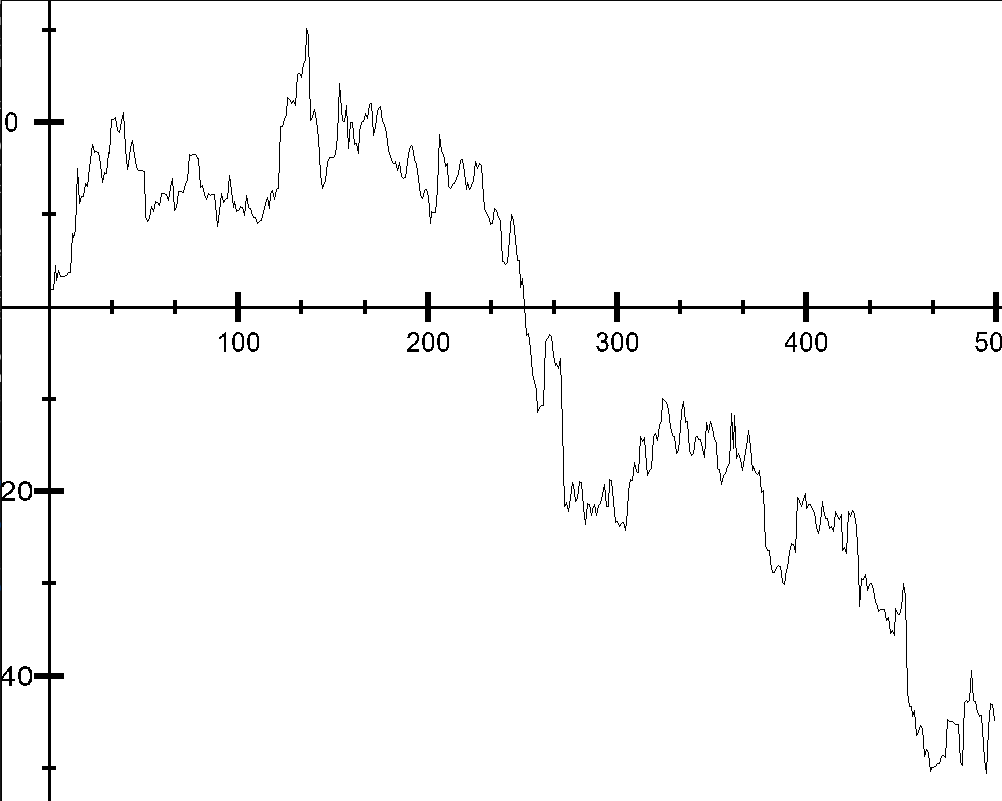
\includegraphics[width=0.6\linewidth]{img/simulation_1D.png}}
    \caption{Evolution d'une simulation au cours du temps}
\end{figure}

\begin{figure}[h] 
    \label{figure2}
    \centering{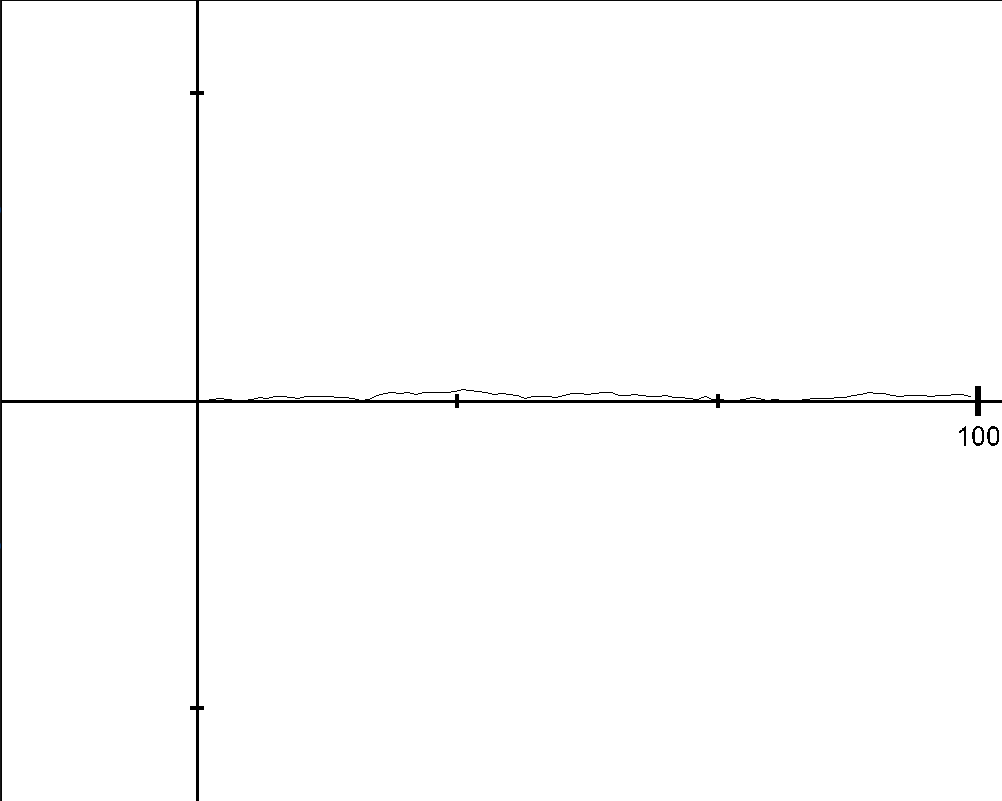
\includegraphics[width=0.6\linewidth]{img/median_1D.png}}
    \caption{Moyenne des tracés au cours du temps}
\end{figure}

\begin{figure}[h] 
    \label{figure3}
    \centering{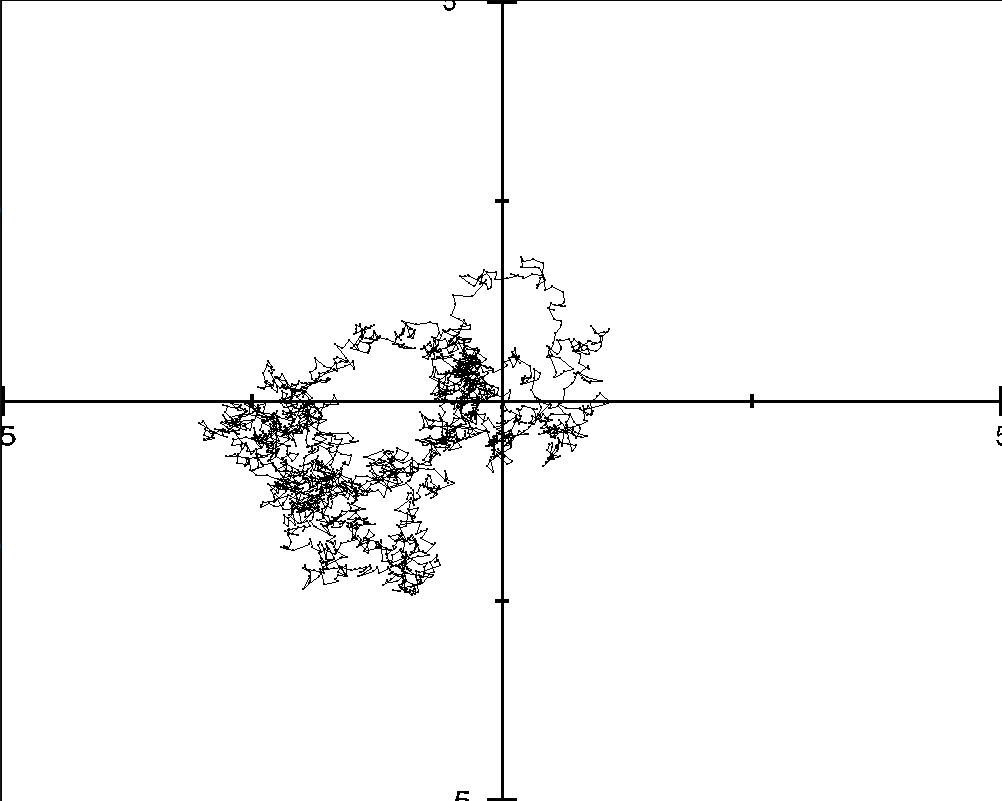
\includegraphics[width=0.6\linewidth]{img/simulation_2D.png}}
    \caption{Une simulation en deux dimensions}
\end{figure}

\begin{figure}[h] 
    \label{figure4}
    \centering{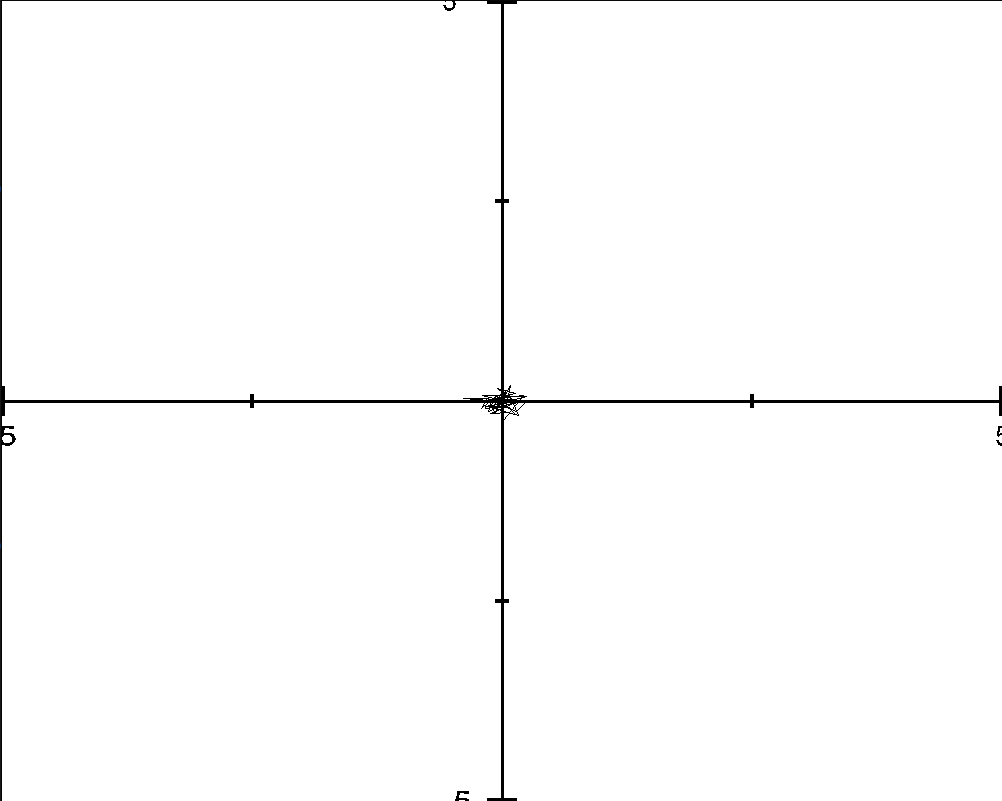
\includegraphics[width=0.6\linewidth]{img/median_2D.png}}
    \caption{La moyenne des simulations en 2D}
\end{figure}

\begin{figure}[h]
    \label{figure5}
    \centering{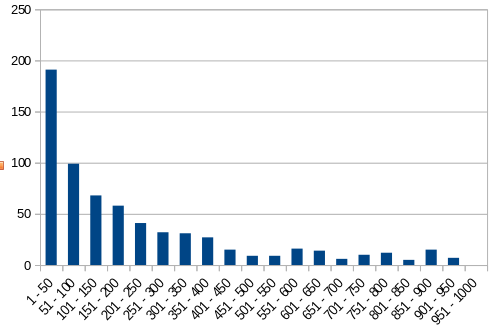
\includegraphics[width=0.6\linewidth]{img/histogram.png}}
    \caption{Un exemple d'histogramme pour 10000 simulations, une marge d'erreur de 0.2, avec 9321 points n'ayant pas atteints l'objectif en moins de 1000 coups}
\end{figure}
\end{document}